% !TEX root = /Users/kartikgohil/Documents/Imperial/Year4/Project/Docs/Final_Report/report_tex/main.tex
\section{Appendices}
\appendix

\section{Circuit Diagrams} \label{Circuit Diagrams}


\subsection{Circuit Diagram for HC-06 Bluetooth Module to Arduino Connection}
\label{arduinobluetooth}
\begin{figure}[H]
\centering
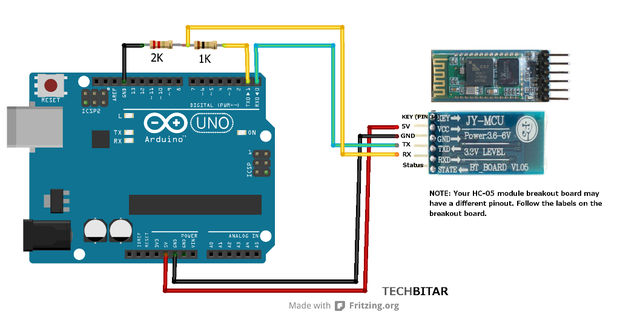
\includegraphics[scale = 1]{Images/arduinobluetooth}
\caption*{Image Available from Reference~\cite{arduinobluetooth}}
\end{figure}

\subsection{Circuit Diagram for Prototype 0.2.03 - Finger Board}
\label{fingerboardsch}
\begin{figure}[H]
\centering
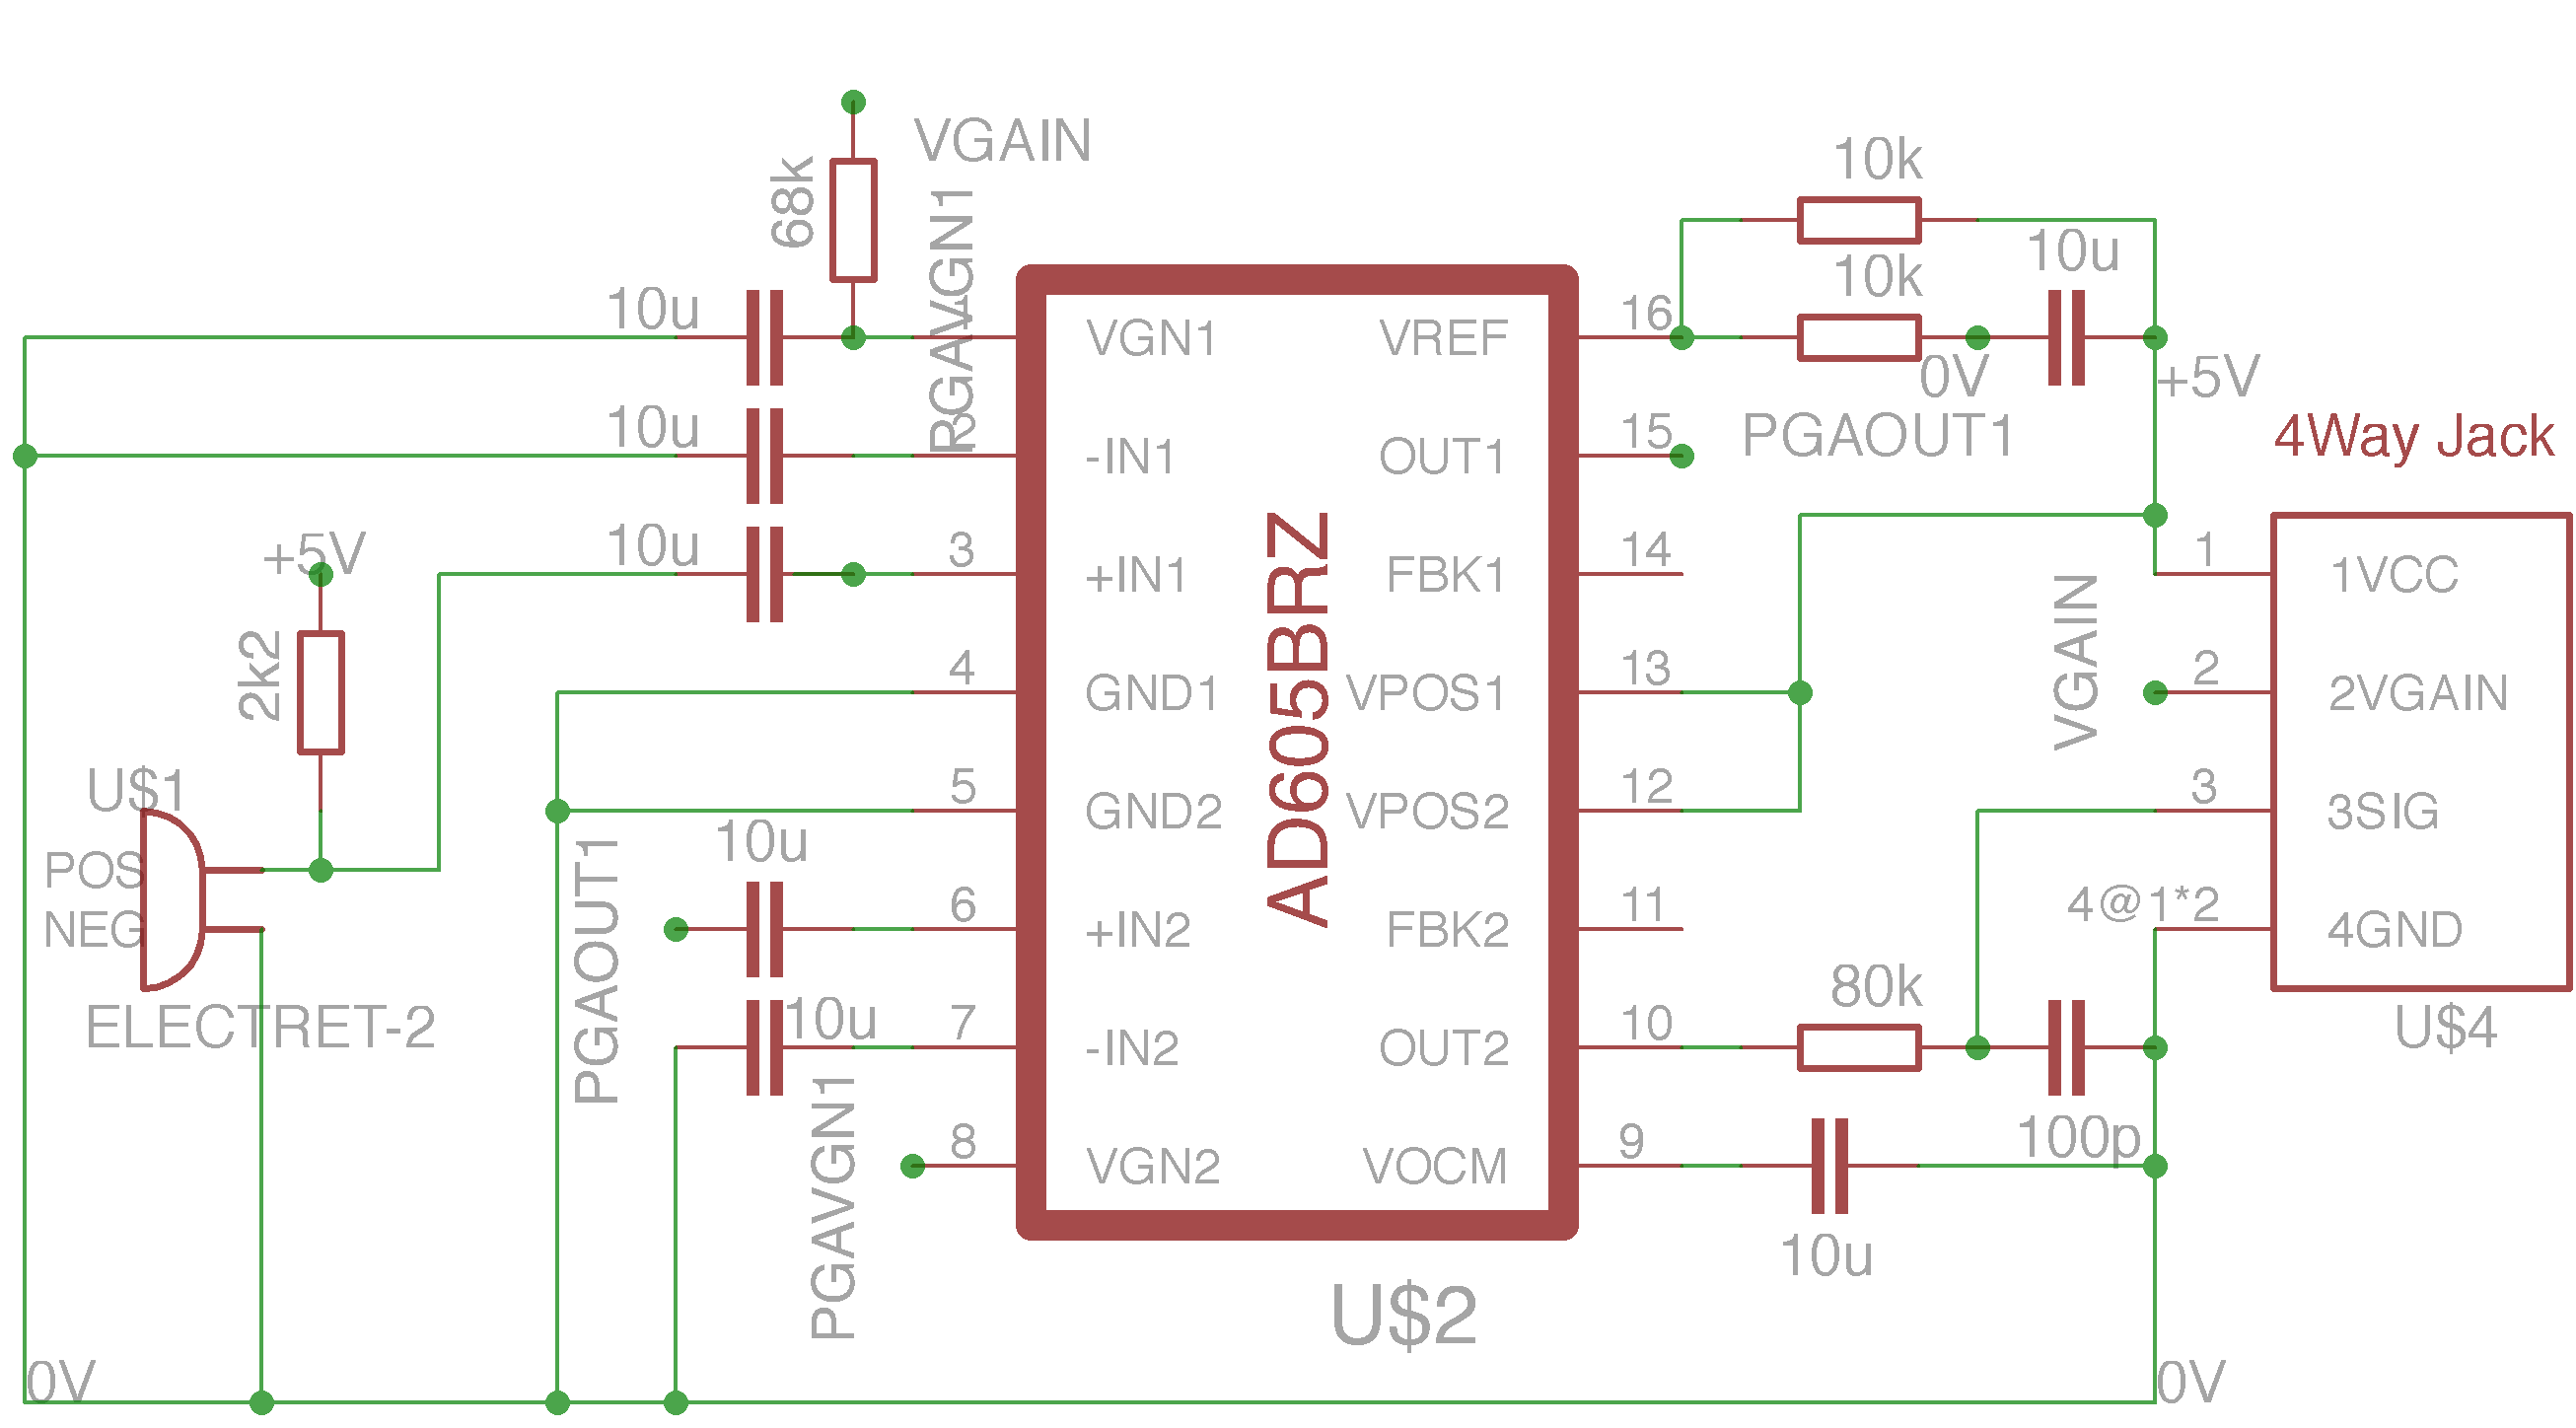
\includegraphics[scale = 1]{Images/mic_schematic_01}
\end{figure}

\subsection{Circuit Diagram for Prototype 0.2.03 - Arduino Shield Version 1}
\label{ardshieldsch}
\begin{figure}[H]
\centering
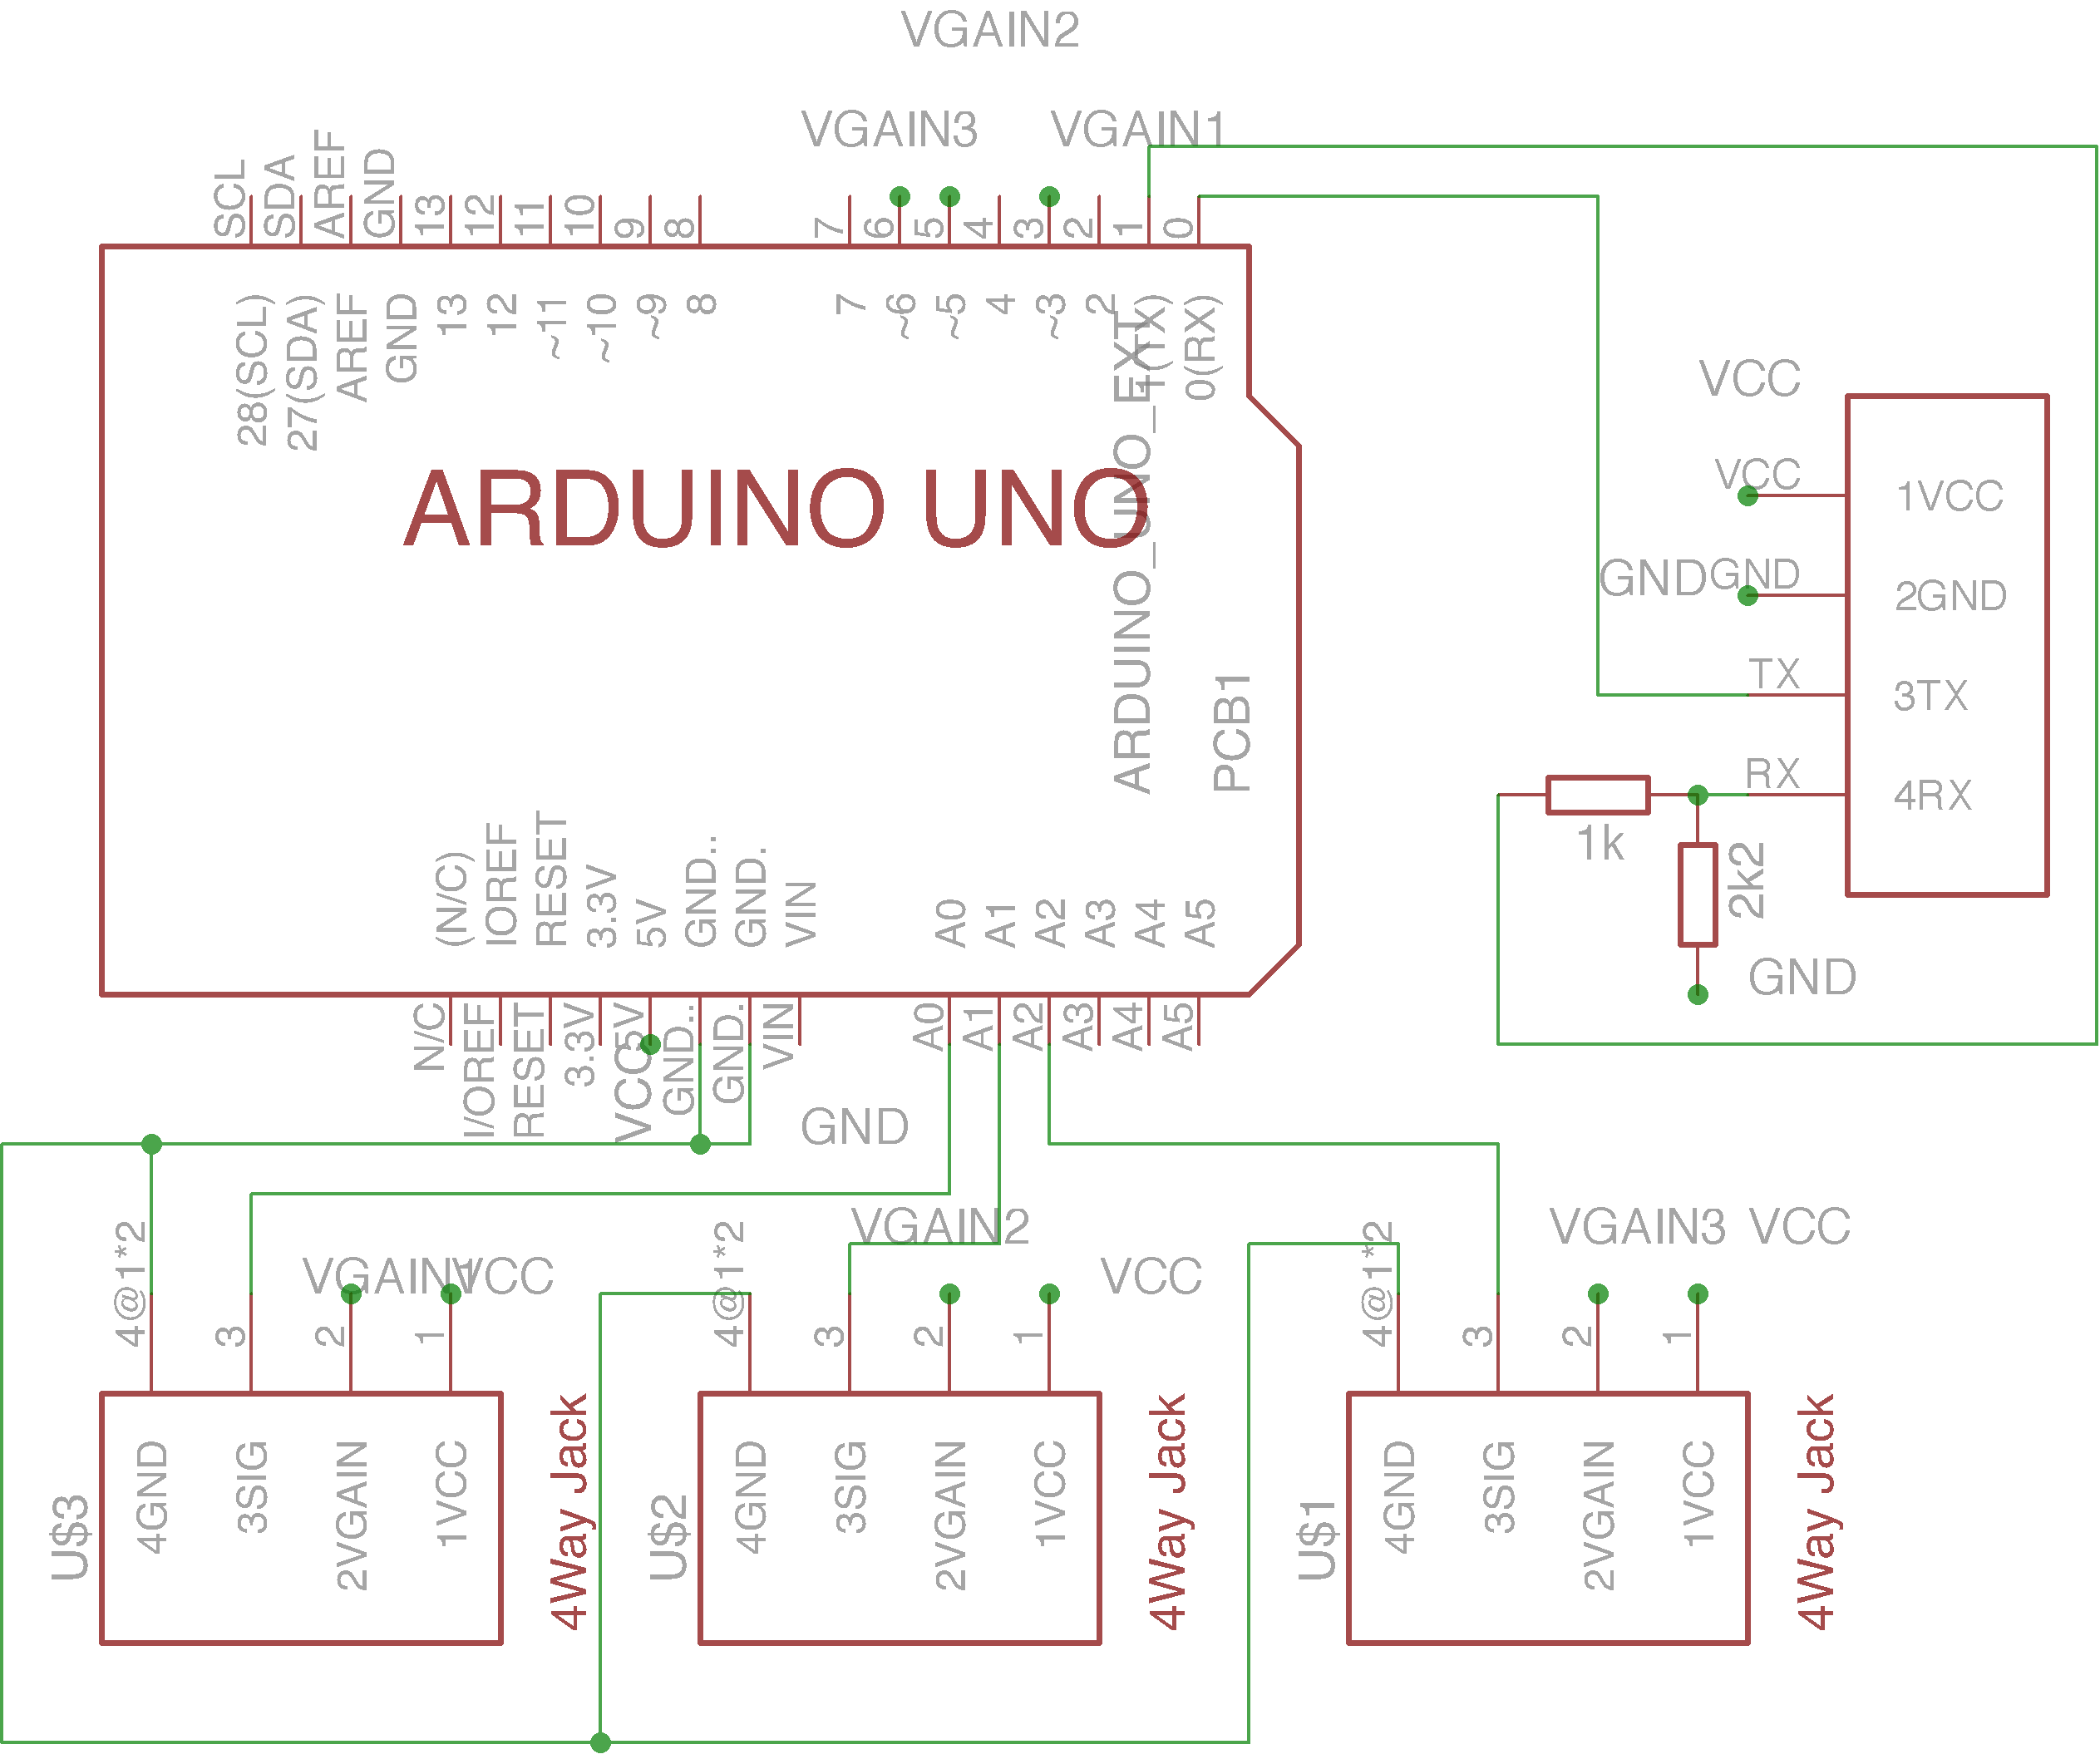
\includegraphics[scale = 1]{Images/ard_schematic_01}
\end{figure}



\section{Flow Diagrams} \label{Flow Diagrams}

\subsection{Flow Diagram for Microcontroller Program, Prototype 0.1.01}
\label{mcflow}
\begin{figure}[H]
\centering
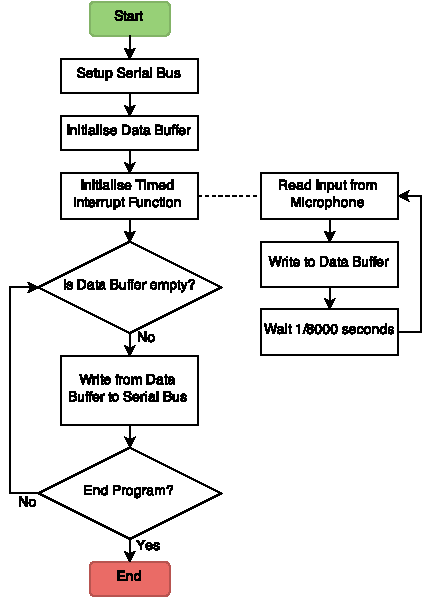
\includegraphics[scale = 1]{Images/mc0101}
\end{figure}
The microcontroller uses timed interrupts to call a function which samples the incoming microphone signal and stores the data to a buffer. The main loop of the program writes the sample data to the Serial bus. 


\newpage
\subsection{Flow Diagram for Interface Program, Prototype 0.1.01}
\label{interfaceflow}
\begin{figure}[H]
\centering
\subfloat['Voice' Mode Program]{
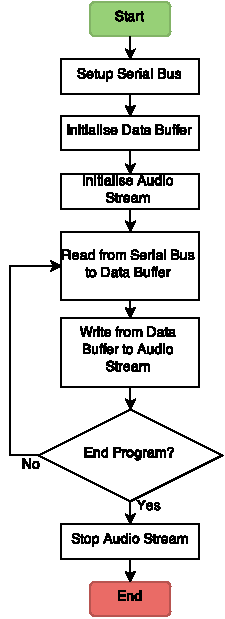
\includegraphics[scale = 1]{Images/interfacevoiceflow}
}
\hspace{72pt}
\subfloat['Sample' Mode Program]{
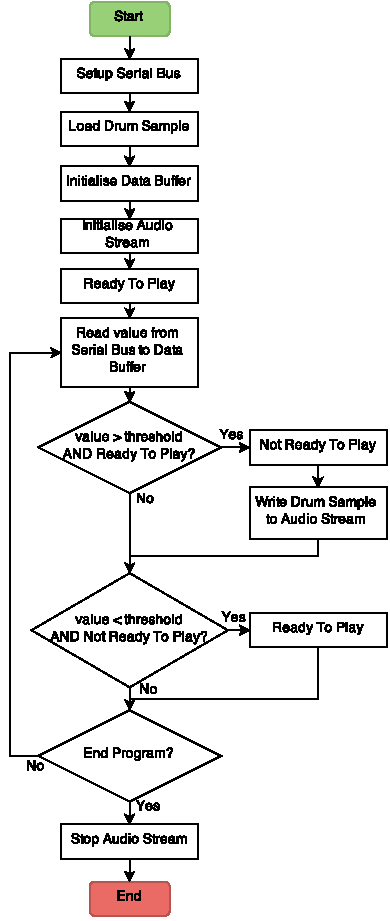
\includegraphics[scale = 1]{Images/interfacesampleflow}
}
\end{figure}
Two Python programs were written to perform the 'Voice' mode and 'Sample' mode separately. The flow diagrams show how these modes work. The 'Voice' mode simply reads samples and writes them to the audio stream, but the 'Sample' mode processes the signal to check whether it has passed a certain threshold to trigger a drum sample. 

\subsection{Flow Diagram for Interface Program, Prototype 0.1.02}
\label{pyblue_flow}
\begin{figure}[H]
\centering
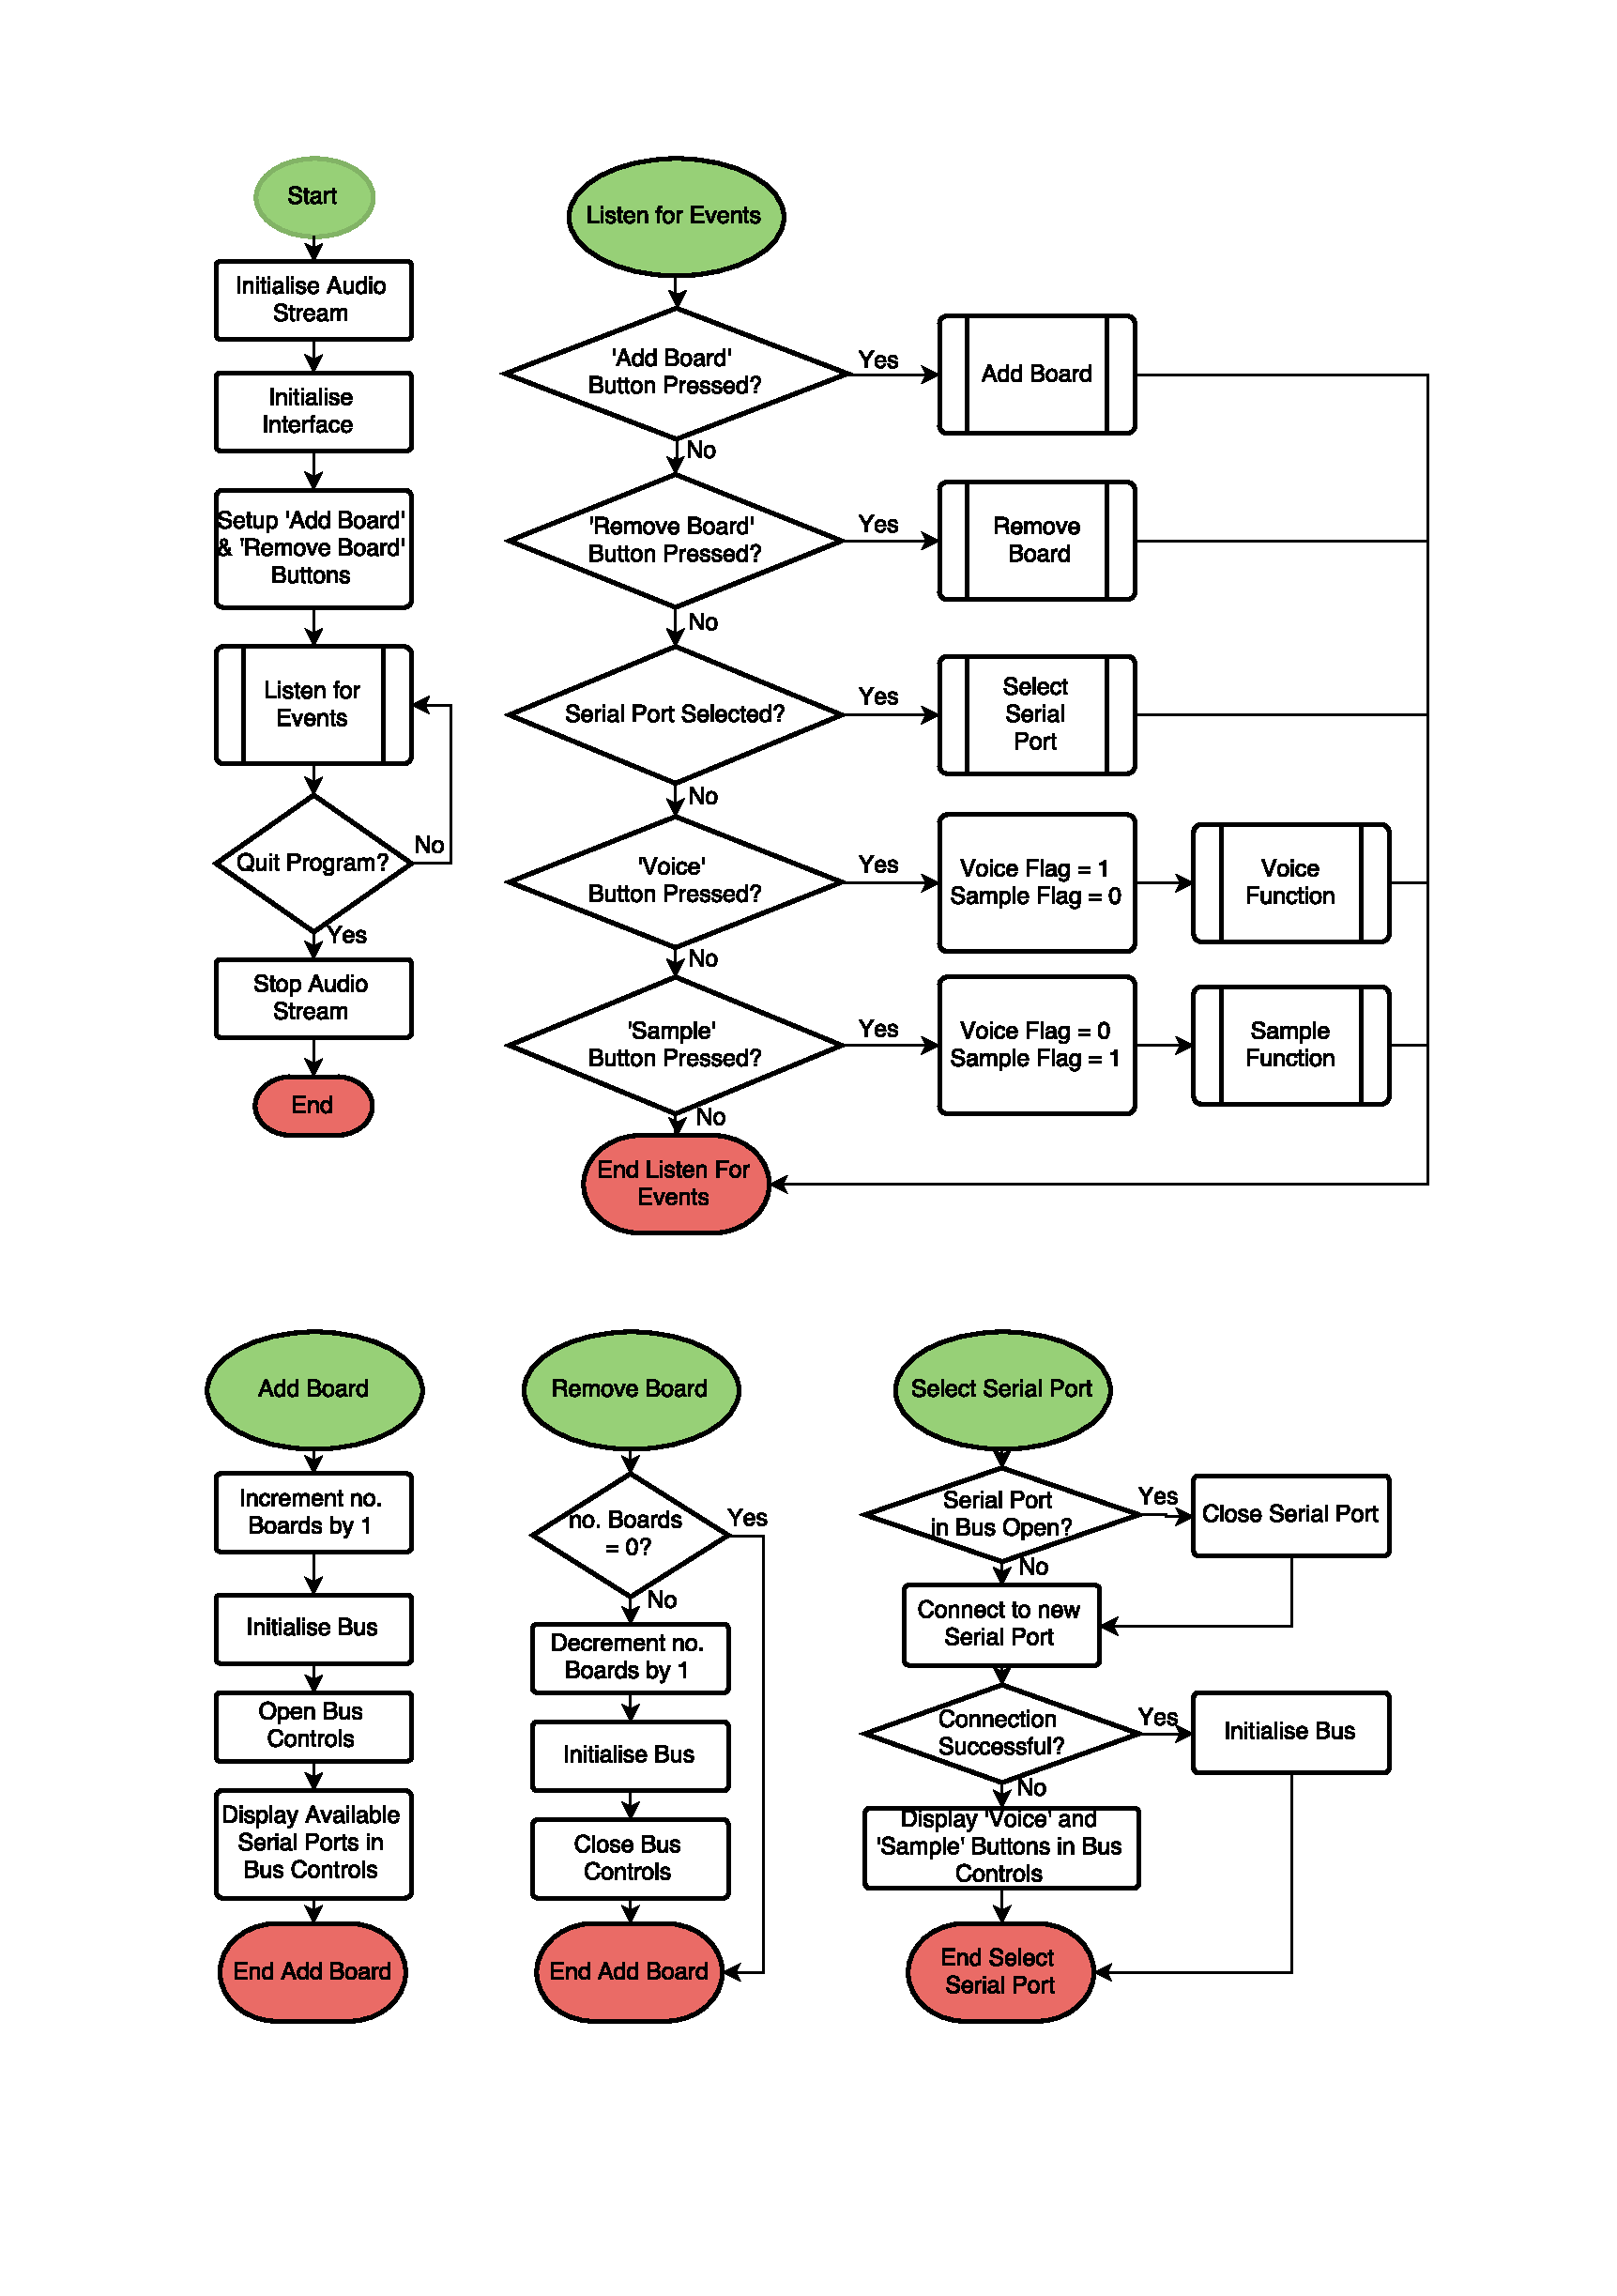
\includegraphics[scale = 0.6]{Images/PyFlow}
\end{figure}
A single Python program was written with a Graphical User Interface (GUI) to give the user basic controls. The flow diagram highlights how the GUI program works, what function is called when a graphical element is interacted with, and how the 'Voice' mode and 'Sample' mode functions are triggered. 


\subsection{Flow Diagram for Interface Program, Prototype 0.2.01}
\label{juceflow}
\begin{figure}[H]
\centering
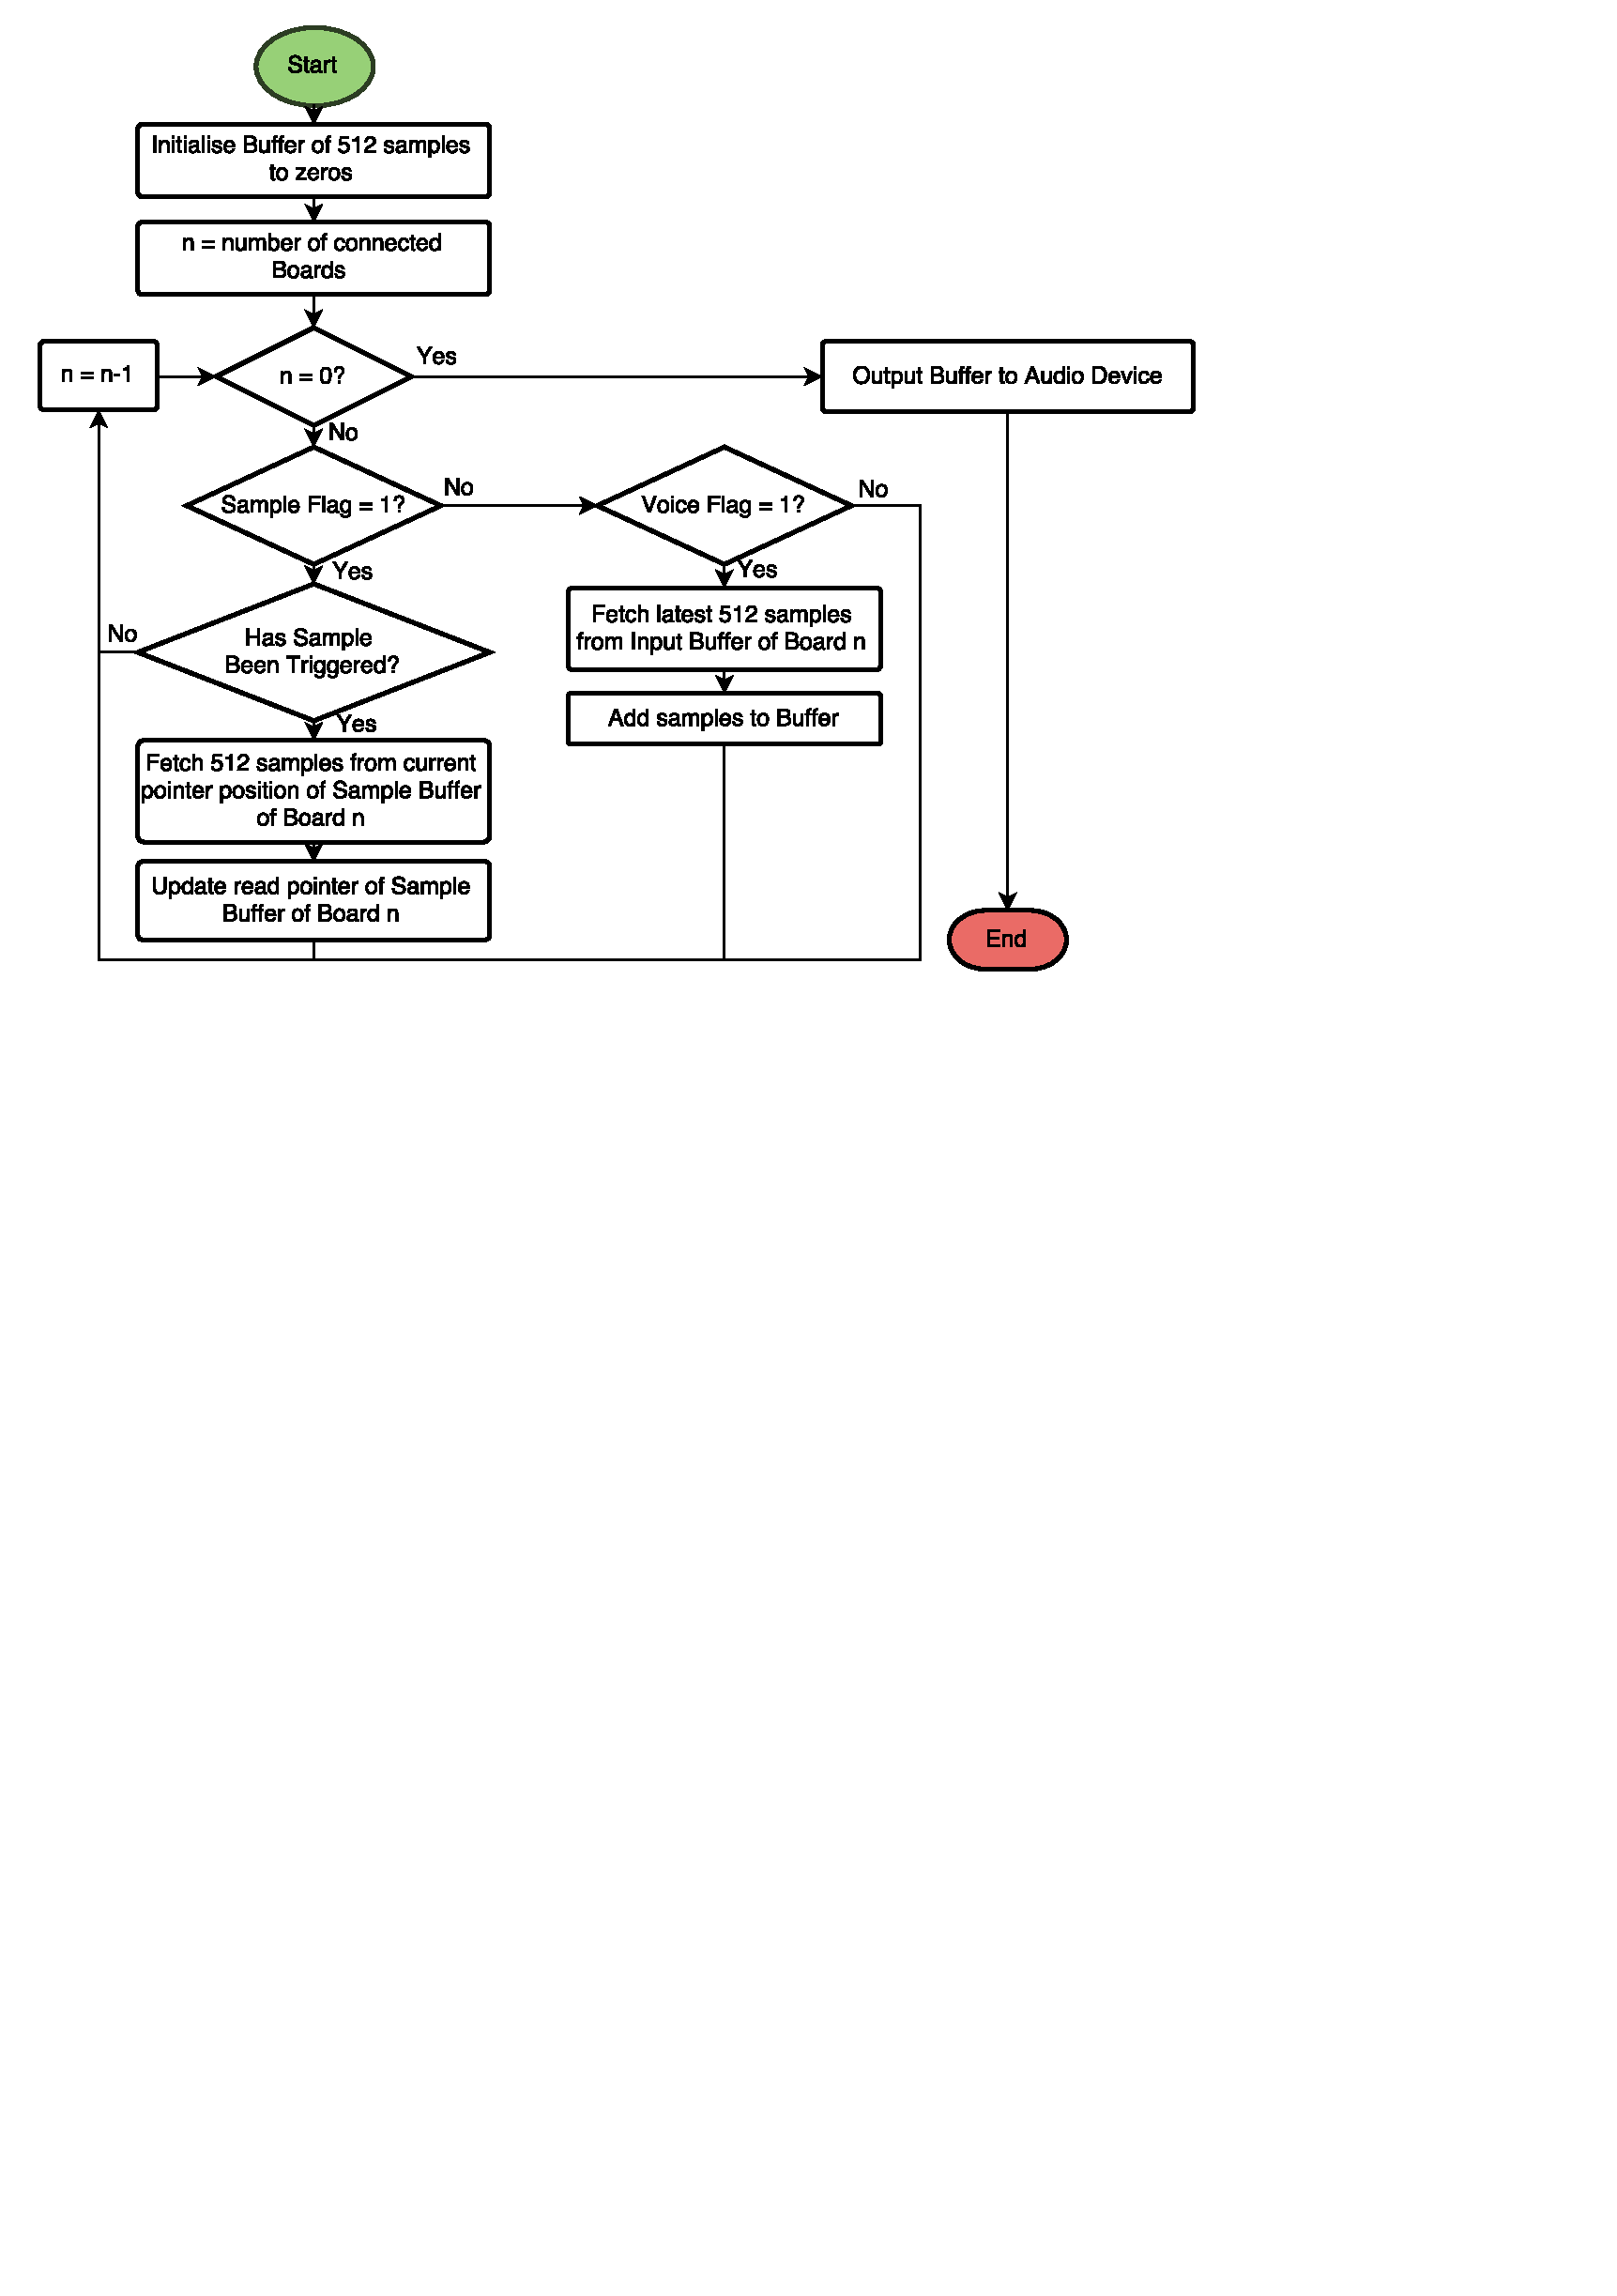
\includegraphics[scale=0.7]{Images/JuceFlow}\\
\end{figure}
The JUCE program consisted of a top-level function that requested 512 data samples on a recurring timer to pass to the audio device. This flow diagram shows how data was transferred between the various classes for a number of Boards operating individually in 'Voice' or 'Sample' modes. 


\section{PCB Design}

\subsection{Finger Board}
\label{fingerboardpcb}
\begin{figure}[H]
\centering
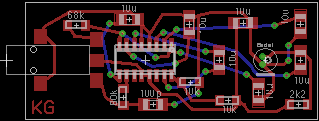
\includegraphics[scale = 2]{Images/mic_pcb_02}
\\ Dimensions: 49.51 x 19.99 mm
\end{figure}

\subsection{Arduino Shield Version 1}
\label{ardshieldpcb}
\begin{figure}[H]
\centering
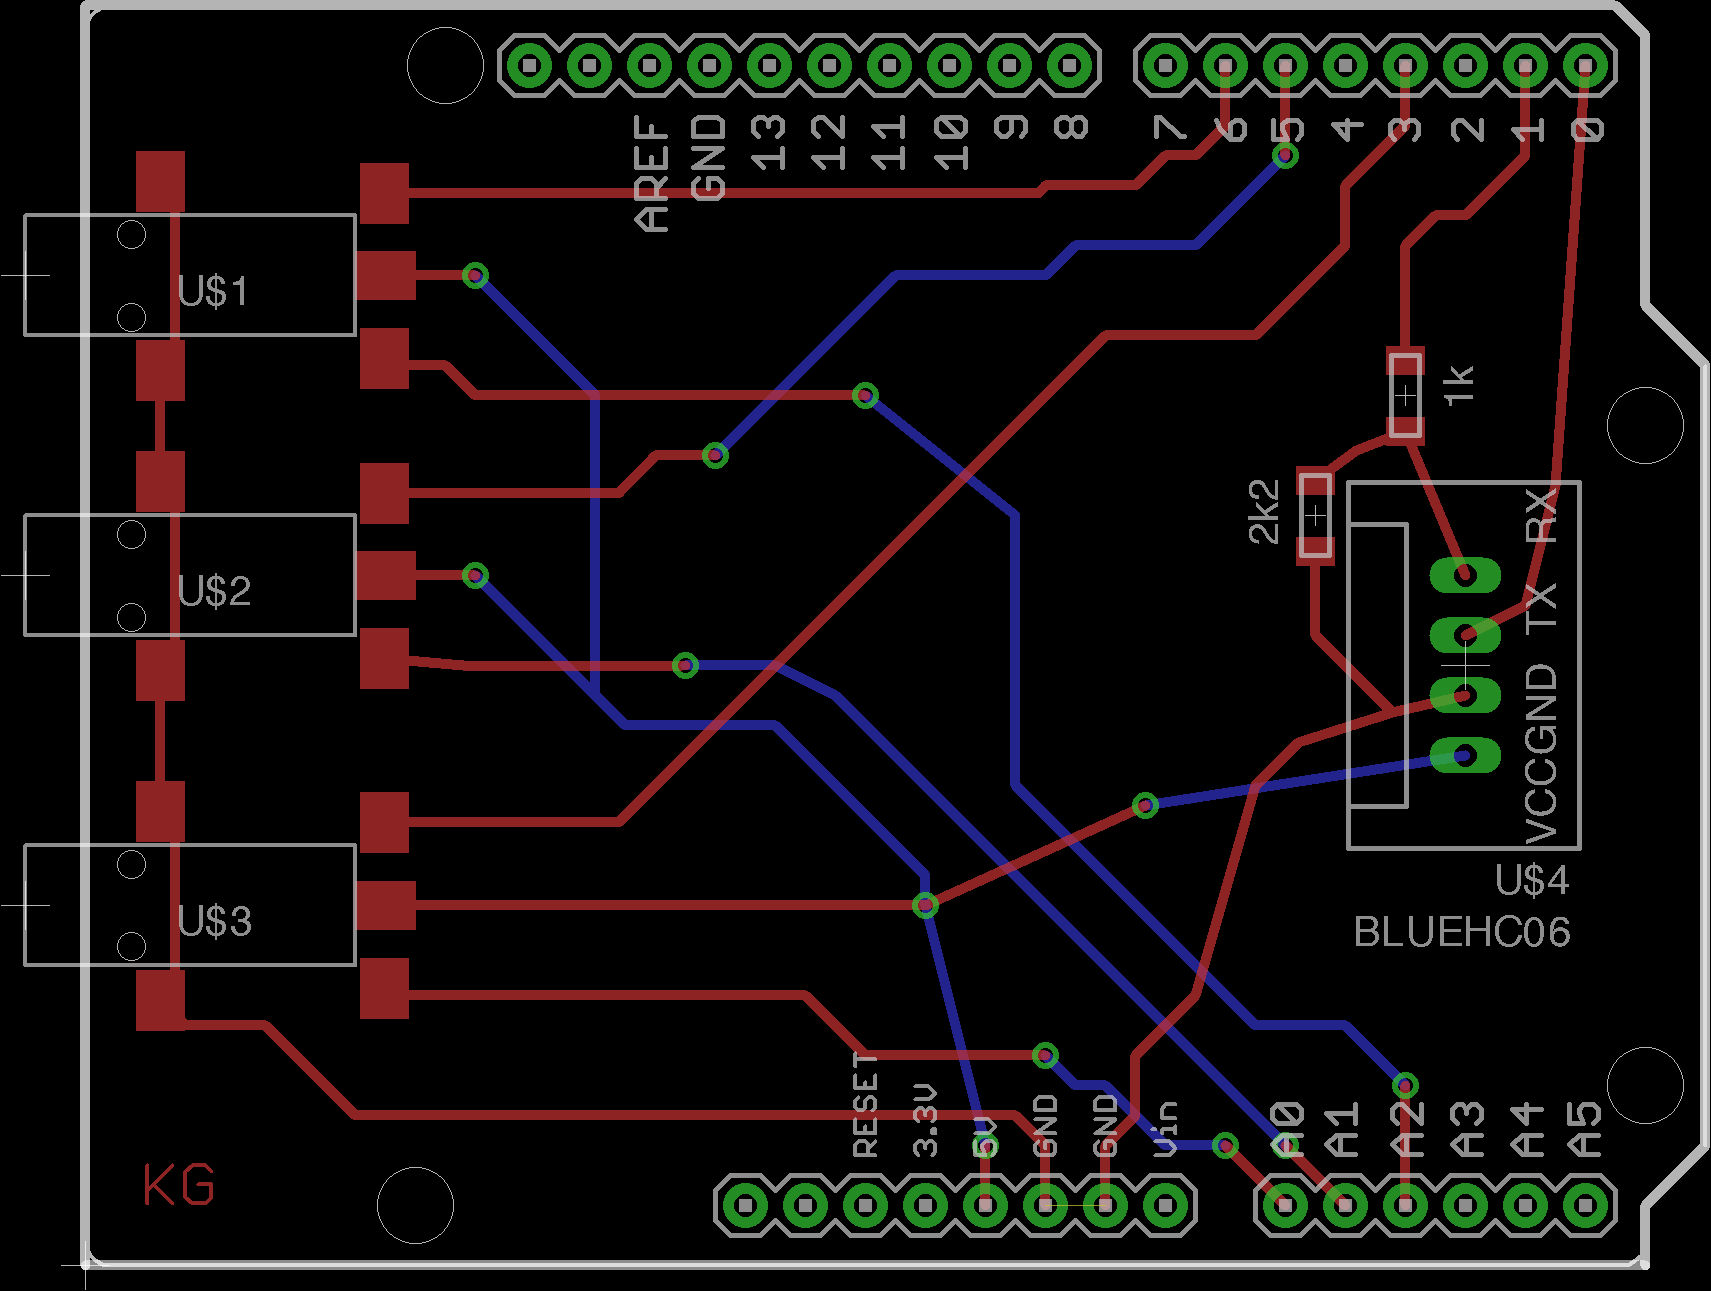
\includegraphics[scale = 1.5]{Images/ard_pcb_01}
\\ Dimensions: 68.58 x 53.34 x 2.5mm
\end{figure}

\subsection{Arduino Shield Version 2}
\label{ardshieldpcb2}
\begin{figure}[H]
\centering
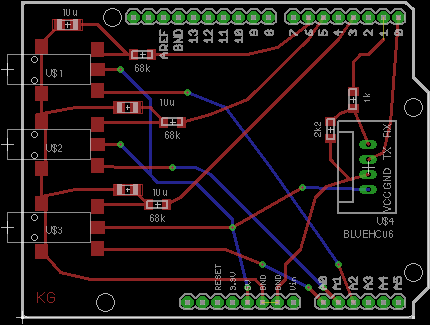
\includegraphics[scale = 1.5]{Images/ard_pcb_02}
\\ Dimensions: 68.58 x 53.34 x 2.5mm
\end{figure}


\section{GitHub Repository} \label{GitHub}

Documentation for this project including all versions of code, 3D models, circuit designs, report drafts, Matlab simulations, etc. can be found in the following GitHub Repository: https://github.com/kartikg33/imp\_fyp\_2015



